\chapter{Introdução\label{chap:Introducao}}

O mercado global de animação e jogos foi avaliado em \$122.20 bilhões em 2010 e é esperado que esta cifra atinja  \$242.93 bilhões em 2016. Esse mercado global pode ser dividido em mercados específicos voltados para a Educação, o Desenvolvimento para Web e a Animação para Entretenimento, podendo esse último ser ainda subdividido em várias categorias \cite{animationMarketSize}, sendo \textbf{Filmes} e \textbf{Efeitos Visuais} categorias de especial interesse para este trabalho. 

Uma tarefa recorrente dentro da indústria cinematográfica é a modelagem e animação de objetos tridimensionais. Tais objetos não estão sujeitos às restrições do mundo físico e permitem gerar cenas e movimentos dificilmente filmados de outra forma. Mesmo em produções com atores reais as técnicas de Animação Computacional se fazem presentes, seja transformando o cenário do filme, projetando sobre o ator uma textura que modifica suas feições ou adicionando à obra um personagem completamente digital. Presentes em praticamente qualquer novo \textit{blockbuster}, as técnicas de animação tridimensional ainda apresentam custos elevados e proibitivos para certas aplicações.

O orçamento para a produção de um filme inclui custos de pré-produção, filmagem, pós-produção e divulgação, devendo-se levar em conta os direitos pelo roteiro, salários dos atores, salários da equipe de produção, construção do set de filmagens, efeitos especiais, figurino e tudo o mais \cite{movieProductionCost}. Apesar da Animação Computacional diminuir o custo de alguns dos componentes citados, ela é em si uma técnica cara. Dessa forma, ao passo que a animação computacional  reduz custos com montagem de cenários e até mesmo maquiagem, muitas vezes um único quadro de um filme pode requerer a animação de milhões de partes móveis. No filme \textit{Monstros SA (2001)}, por exemplo, foram utilizados mais de 2 milhões de fios de cabelo individualmente nomeados para a construção do personagem Sully. Um único quadro com o personagem custou em média de 11 a 12 horas de trabalho criativo \cite{sullyExample}. Com tantas horas de trabalho criativo gastas durante o processo de animação, é evidente a necessidade do desenvolvimento de técnicas que auxiliem os animadores.

Uma técnica importante que vem ao auxílio dos animadores consiste em transferir movimentos e expressões de um ator para um modelo computacional. Metodologias para captura ótica de performance teatral capazes de registrar
expressões de um ator em geometria detalhada são utilizadas na indústria já há
algum tempo. Exemplo conhecido do uso dessa tecnologia é o personagem \textit{Gollum} no
filme \textit{O Senhor dos Anéis: A Sociedade do Anel } (2001), onde o ator Andy Serkis
utiliza uma roupa especial com marcadores visuais durante as gravações para que
mais tarde a equipe de efeitos visuais renderize sobre ele um modelo
computacional tridimensional da criatura amaldiçoada. Mais recentemente, a mesma
tecnologia - em estado aprimorado e muito mais rica em detalhes - é utilizada em
\textit{O hobbit} (2015), onde o ator Benedict Cumberbatch dá vida ao dragão Smaug. A Figura \ref{fig:smaug} ilustra o processo. Na Figura \ref{fig:smaugA} observa-se o modelo que está sendo animado pela performance do ator. Na Figura \ref{fig:smaugB} mostra-se em detalhes pontos colocados no rosto do ator para auxiliar a captura de expressões. 

\begin{figure*}[!htb]
   \centering
 \begin{subfigure}[]{\label{fig:smaugA}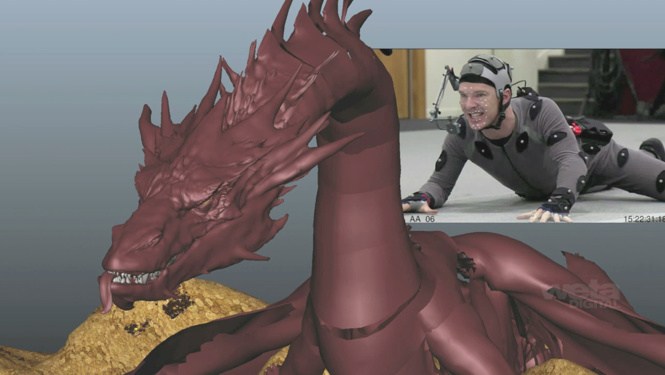
\includegraphics[width=0.4\linewidth]{./figs/exemploSmaug.jpg}}
  \end{subfigure}   
   \begin{subfigure}[]{\label{fig:smaugB}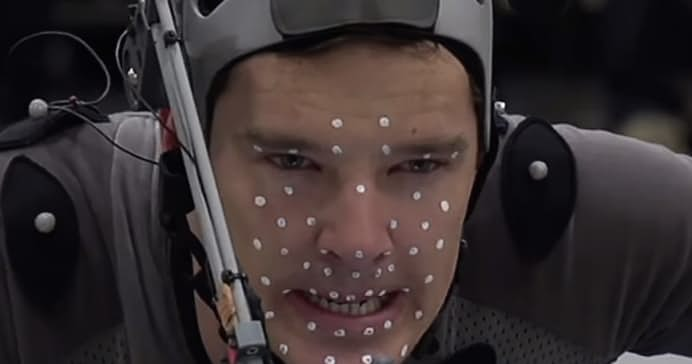
\includegraphics[width=0.4\linewidth]{./figs/Smaug_Benedict.jpg}}
  \end{subfigure}   
    \caption{Exemplo de utilização de captura de movimentos e expressões 
    na indústria cinematográfica. Pontos cuidadosamente colocados no rosto
  do ator são utilizados para transferir expressões para o modelo 
  tridimensional do personagem (retirado de \cite{sherlocksmaug}).}
    \label{fig:smaug}
\end{figure*}

Nesse tipo de aplicação cinematográfica requer-se do sistema de animação computacional uma alta precisão no
ajuste do modelo computacional ao ator em cena. Para esse fim, utilizam-se
ambientes especiais onde a iluminação é controlada e marcadores visuais no cenário e no ator, sendo que muitas vezes a captura da imagem é feita por
um arranjo de câmeras ou ainda por câmeras de alta resolução. Além disso, o resultado do processamento
recebe um ajuste fino realizado por vários artistas para que o resultado
apresentado seja o mais convincente possível. Vale notar que não é possível realizar esse ajuste fino caso não haja um longo prazo disponível entre a captura da imagem e o instante em que os resultados precisam ser apresentados ao público.

Outro recurso utilizado para a animação auxiliada por captura de vídeo é o uso de fantoches digitais, mas neste caso os
requisitos de tempo são muito mais severos. Nessa
aplicação, vista em programas televisivos e em parques de diversão ao redor do
mundo, um ator em uma câmera escondida anima em tempo real um modelo renderizado
em projetor e responde ao vivo às perguntas do público. O personagem animado
apresenta expressões corporais e faciais que encantam o público, deixando os
mais novos convencidos de que conversaram com seu personagem preferido e os mais
velhos se perguntando como aquilo pode ser possível. Nessa aplicação, os requisitos de tempo são muito mais severos, devido ao tempo de resposta
curto necessário para a interação entre público e personagem digital, não é
possível o ajuste fino dos artistas, mas ainda sim é possível fazer uso de
iluminação controlada, câmera(s) de alta qualidade e marcadores visuais. A
equipe por trás do personagem pode ainda fazer uso de controles pré-programados.

Apesar das soluções existentes apresentarem resultados adequados para as aplicações citadas, elas apresentam um alto custo. Dessa forma, ainda que grandes empresas se disponham a bancar o preço da tecnologia atual, ele se torna proibitivo para aplicações desenvolvidas por pequenas empresas. Portanto, o surgimento de produtos que realizem as mesmas
tarefas a custos mais baixos é certamente de interesse do mercado global de animação. Tal produto
poderia, por exemplo, ser utilizado por animadores independentes para acelerar seus projetos. A motivação inicial deste trabalho foi justamente a de atender esses animadores independentes.

Pode-se observar, ainda, que programas de televisão educacionais para crianças abundam no mercado, mas são em sua maioria
direcionados ao público infantil geral. Um nicho não atendido é o de
crianças autistas. Apesar das dificuldades encontradas por essas crianças
variarem muito de um indivíduo para o outro, é comum que crianças autistas
apresentem dificuldade em manter contato visual, mesmo que seja com personagens
de um filme. Assim sendo, as animações convencionais não são adequadas para esse público e há certamente motivação para o desenvolvimento de desenhos infantis próprios para as crianças autistas.

Uma empresa interessada em desenvolver tais animações muito provavelmente não objetiva fins lucrativos, mas sim busca realizar um interesse social. Logo, a empresa dificilmente terá os mesmos recursos financeiros de uma que trabalhe com o público geral e não poderá arcar com os custos envolvidos.  Uma das motivações deste trabalho é que o produto desenvolvido possa ser utilizado como ferramenta para auxiliar o desenvolvimento de programas infantis com foco em crianças autistas.

O Capítulo 2 deste trabalho discorre sobre a fundamentação teórica 
por trás das técnicas utilizadas. Reconhecimento de pontos do rosto,
renderização de objetos tridimensionais, filtragem digital e estimação de
profundidade são tópicos abordados. No Capítulo 3 as técnicas introduzidas são relacionados para compor a metodologia da aplicação proposta neste trabalho.
No Capítulo 4 os resultados obtidos são apresentados e discutidos.
O último capítulo elabora conclusões e aponta propostas de melhorias futuras para o
trabalho.
